\documentclass[a4paper,11pt]{report}
\author{Michael Brock}
\title{Getting Started with UAV Software Development}
\usepackage{fancyhdr}
\pagestyle{fancy}
\usepackage[margin=1.5in]{geometry}
\renewcommand{\chaptermark}[1]{%
	        \markright{\thechapter\ #1}}
\fancyhf{}  % delete current header and footer
\fancyhead[L,RO]{\bfseries\thepage}
\fancyhead[LO]{\bfseries\rightmark}
\fancyhead[RE]{\bfseries\leftmark}
\renewcommand{\headrulewidth}{0.5pt}
\renewcommand{\footrulewidth}{0pt}
\addtolength{\headheight}{2pt} % space for the rule
\fancypagestyle{plain}{%
	   \fancyhead{} % get rid of headers on plain pages
	      \renewcommand{\headrulewidth}{0pt} % and the line
	  }
    \usepackage{graphicx}
\usepackage{setspace}
\usepackage{microtype}
\usepackage{menukeys}
\usepackage{attachfile}
\usepackage[T1]{fontenc}
\usepackage{lmodern}
\usepackage{fancyvrb} %Allow bold in verbatim text.
\usepackage[section]{placeins} %Deal with floats being in the wrong place.
\usepackage{color}
\definecolor{mygreen}{rgb}{0,0.6,0}
\definecolor{mygray}{rgb}{0.5,0.5,0.5}
\definecolor{mymauve}{rgb}{0.58,0,0.82}

\usepackage{listings}
\AtBeginDocument{\renewcommand{\thelstlisting}{\thesubsubsection.\arabic{lstlisting}}}
\def\l@lstlisting#1#2{\@dottedtocline{1}{3em}{3.5em}{#1}{#2}}
\lstset { 									%
%	language={[ANSI]C}, 					%
	otherkeywords={printf, strcpy, *, &, malloc},	%
	numbers=left, 							%
	numberfirstline=true,					%
	showspaces=false, 						%
	showtabs=false, 						%
	showstringspaces=false, 				%
	commentstyle=\color{mygreen}, 			%
	tabsize=4, 								%
	keywordstyle=\color{blue}, 				%
	xleftmargin=2em,						%
	extendedchars=true,     			    %
	basicstyle=\small\sffamily,				%
	columns=fullflexible,					%
	breaklines=true,		            	%
	stringstyle=\color{mymauve}}
\lstloadlanguages{C}
\lstloadlanguages{Java}
\lstloadlanguages{bash}
%Sorting code floats.
\usepackage{float}
\floatstyle{plain}
\newfloat{code}{htb}{loc}[chapter]
\floatname{code}{Code Example}
\renewcommand{\abstractname}{Introduction}
\interfootnotelinepenalty=10000
\setcounter{secnumdepth}{1}
\setcounter{tocdepth}{1}
\makeatletter
\usepackage{parskip}
\renewcommand*{\listof}[2]{%
	\@ifundefined{ext@#1}{\float@error{#1}}{%
		\expandafter\let\csname l@#1\endcsname \l@figure  % <- use layout of figure
		\@namedef{l@#1}{\@dottedtocline{1}{1.5em}{2.5em}}%
		\float@listhead{#2}%
		\begingroup
			\setlength\parskip{0pt plus 1pt}%               % <- or drop this line completely
			\@starttoc{\@nameuse{ext@#1}}%
		\endgroup}}
\makeatother
\usepackage{hyperref}

\begin{document}
\maketitle
\tableofcontents
\begin{abstract}
  This getting started guide is being written with the intent of offering those interested in developing software for Unmanned Aerial Systems.
  It also serves as an introduction to some of the hard skills that are required in an Electrical Engineering or Information Technology degrees.

  Due to the nature of the programs utilized, this book will utilize Fedora as a base operating system (OS).
	Given this requirement, you may find that some parts of the book will ask you to look at others prior to moving on. This book is intended to be a linear in terms of how it is read; however sometimes skipping ahead before coming back will offer a great benefit.
	I will highlight this at the relevant sections in the book, but expect it most in the first chapter.
  Whilst it is possible to use a Windows OS for software development, Linux was chosen due to the ease of installation of the C/C++ toolchain for ARM development.
  Therefore the initial part of this book will focus on the setup and basic use of a Linux based OS. The caveat to this is that while some basics of linux will be covered, it will not be explained in detail. This is not a "Learn Linux in 10 Seconds" guide.

  This book will focus on the development of software in two languages, initially Java to get familiar with Object Oriented concepts, then C/C++ as this is what is used in most UAS systems.
  The Java section of the book is most relevant to Electrical Engineers and Information Technology students studying at university, as it is the most common language taught.
  However in terms of this training continuum, C/C++ are the main focus after the student has a base understanding of Object Oriented concepts and syntax.

  So without further ado; good luck, have fun and enjoy the pages that follow.

\end{abstract}

\chapter{Toolchain Setup}
  \label{ch:ToolchainSetup}
  Getting our toolchain setup ready for software development can be a tricky task.
  A lot of things need to be considered when setting up your toolchain. The first is your base OS.
  This can heavily influence the ease of use and efficiency of you programming workflow.
  An OS that must be forced to incorporate a conglomerate of mismatched tools will only hinder you as you progress through this guide.

  Linux is the OS we will be using in this guide. Whilst chances are you may not have been exposed to much in the way of Linux distros (distributions), I will endeavor to make this as painless as possible.

  \section{Setup}

  The setup of a Linux distro can be done in one of a couple ways. If you have a spare computer lying around then you can install it on that, else you can install it on your existing computer in a bit of software know as a virtual machine.
  For the sake of this guide I will assume you are running Windows. On the off chance you own a Mac, then I recommend Google to find resources on installing VMs on there.

  \subsection{Virtual Machine Setup}
    There are a variety of virtualisation software packages out there, each with their own advantages and disadvantages.
    This guide will utilize one known as VirtualBox. It is by no means the best bit of software out there; however it is free, easy(ish) to use and has no major disadvantages for the purposes of this text.
    If you wish to use another virtualisation package feel free to do so, but be advised my ability to help you may be degraded.
    The setup is pretty straightforward and I'll guide you through it below.
    \paragraph{}
    The first step is to download the installation media from the VirtualBox website. \url{https://www.virtualbox.org/}. Installation should be relatively easy, just follow the bouncing ball after launching the installer, as demonstrated below.

    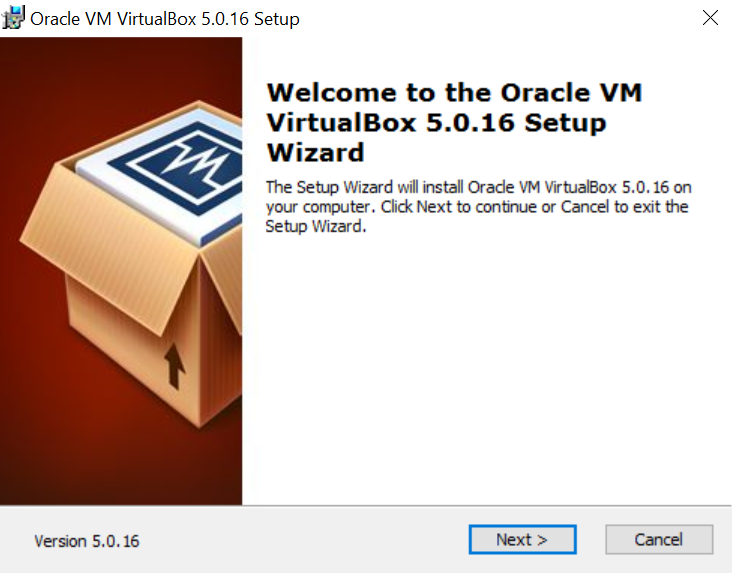
\includegraphics[width=7cm]{vbox1.PNG}
    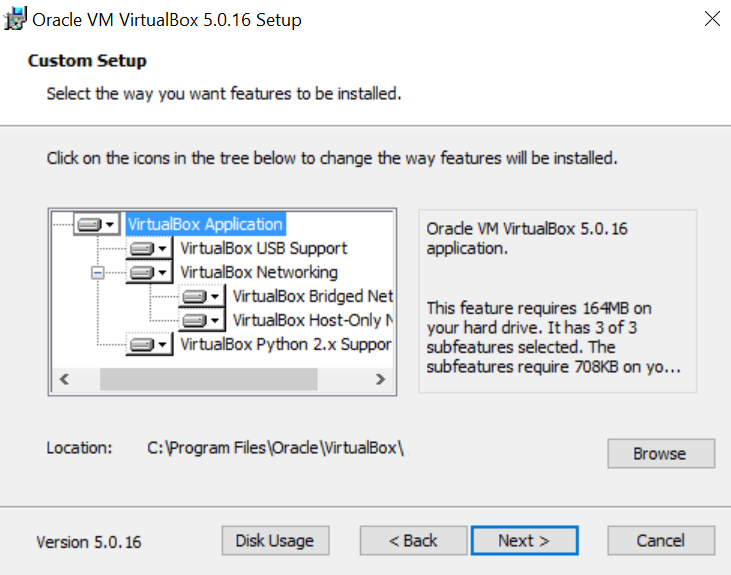
\includegraphics[width=7cm]{vbox2.PNG}
    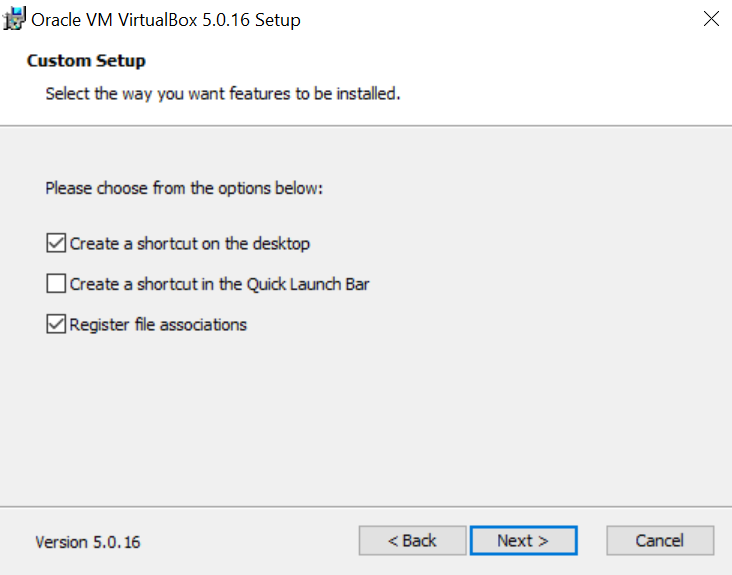
\includegraphics[width=7cm]{vbox3.PNG}
    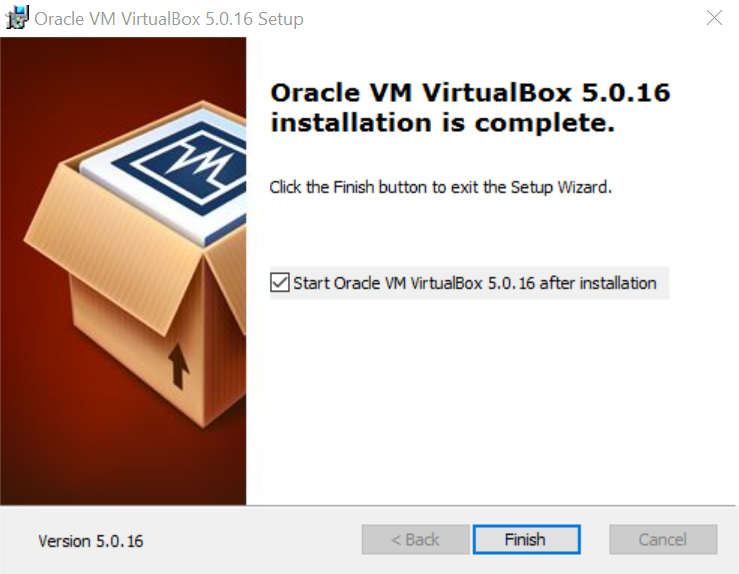
\includegraphics[width=7cm]{vbox4.PNG} \\

    Now that VirtualBox is installed we can go about setting up our VM. The first thing we need is a copy of the operating system. This will usually come in the form of an 'ISO Image'. This file is essentially a disc, but in digital form.
    It contains (usually) everything that will be required for the basic install of the OS. Once again, feel free to use any distro you would like, however the one supported and used by this guide is Fedora Workstation (version 23 at time of writing).
    This can be downloaded from \url{https://getfedora.org/en/workstation/}. However should you wish to download this whilst on a university campus, 1.4GB can be seen to be quite a large download. AARNet offers a mirror of Fedora images here \url{https://mirror.aarnet.edu.au/pub/fedora/linux/releases/23/Workstation/}.
    All you have to choose is which architecture you want to run. If you have a 32 bit system, then you want the 'i386' architecture, 64 bit users will want the 'x86\textunderscore64' architecture.
    You can check whether you are running 64 bit or not by going to control panel and selecting "System and Security" then "System". Labelled as "System Type" your architecture will be listed.\\

		Now we have to install Fedora onto the software\\

		Now download and install some basic packages. (git is the main one here)\\

		Now use git to clone down my repo, and show two methods of install. One is run my script to do it all, the other is to just have a list of packages and go ham.

	\section{Linux Basics}
		Now that we have Fedora configured and setup lets take a look around.

		\subsection{Main User Interface}
			Intro to the GNOME3 interface and customizing it.

		\section{CLI Basics}
			The command line is pretty much as bare bones as you can get in terms of user interface.
			However the lack of pretty buttons is offset by the sheer power it has in terms of control of your machine.
			It is also significantly faster in general as it doesn't require the overhead of interpreting user input into a graphical user interface (GUI), let alone the overhead of producing the GUI itself.
			The command line also offers a form of programming known as scripting. This involves storing commands to be executed at a later time in a file.
			The setupToolchain.sh file you ran earlier is an example of a basic script, open it up and have a look if you are curious.
			This section will focus on the bash shell as this is the most common shell to be found on Linux and Unix systems. For a more comprehensive list I recommend you look at \url{https://github.com/jlevy/the-art-of-command-line}
			Here are some of the basic commands you can use in the CLI:
			\begin{description}
				\item[cd]
					This command allows you to change which directory you are in.
					It accepts a single argument which is the directory you want to change into.
					When changing between directories that are more that one 'folder' away, eg. from myFolder through mySubFolder into mySubSubFolder then this is achieved by separating intermediate directories with a '\' character.
					The cd command also makes use of special characters in Linux. The first relevant one is ".", this means the directory you are currently in. Extending this ".." represents the directory above, or parent directory, to the directory you are currently in.
					Example usage 'cd ../../sample/softwareGuide'.

					Another thing I will mention about 'cd' is that if you prefix your argument with '/' then the directory you start in is the root directory. Omitting '/' means that the directory you are changing into is relative to where you currently are.

				\item[ls]
					Think list. The 'ls' command lists the contents of the current directory. Alternatively you can specify a directory and it will list the contents of that directory.
					'ls' also has some useful flags you can set to make the output more readable or relevant to what you are trying to achieve.
					\begin{itemize}
						\item -a (all) shows you all of the files including hidden files
						\item -h (human) gives you a more human readable output
						\item -S (sort) sorts the output by size
						\item -l (long) shows more detail including sizes and permissions
					\end{itemize}
					Example usage "ls -lahS ../otherDir"

				\item[cp]
					Copy, literaly as it sounds lets you copy one thing to another, this can be a file or a directory
					The usage of this command is 'cp <source file/dir> <destination file/dir>'.
					\\Example usage "cp someFile ../newFolder/destFile"

				\item[mv]
					Move, equivalent of cutting and pasting, this will move a file or directory from one location to another.
					Syntactically the same as 'cp' the usage of this command is 'mv <source file/dir> <destination file/dir>'.\\
					Example usage "mv ../someFile currentDirFile"

				\item[rm]
					Remove, this command is your method of deleting files. The most basic usage of this command will only delete files or empty directories and is executed by calling "rm <file/emptyDir>".
					However it also has some nice flags that make it incredibly powerful (remember with great power comes great responsibility. Ensure you don't delete things you shouldn't).
					\begin{itemize}
						\item{-f}
							Force, ignore non-existent files (yes that does happen), never prompt for confirmation
						\item{-i}
							Interactive, this flag will make it prompt you about everything it tries to delete and you can say yes or no
						\item{-r}
							Recursive, this allows you to delete non-empty directories and their contents recursively
					\end{itemize}

					Note that if you use 'rm' to remove a file, it is usually possible to recover the contents of that file.\\

					Example usage "rm -rf thisDirectoryWillSoonBeHistory"

					\item [mkdir]
					Make Directory, this command allows you to create a directory. It has a few flags you may like/need to use.
					\begin{itemize}
						\item[-m] Mode, this sets the mode of the directory where the mode is as it is in chmod
						\item[-p] Parents, create all necessary parent directories
						\item[-v] Verbose, output to the console what the program is doing. (more detail)
					\end{itemize}

					Example usage "mkdir -p newDirectory"

				\item[nano]
					On Linux systems there is usually a variety of text editors available on a machine. In this course, as beginners, I recommend that you use nano.
					It is a more user friendly editor than the more common vim(or vi) however can still be quite powerful.
					You launch it by giving the command "nano <fileToOpen>". However keep in mind the file you are opening does not have to exist at the time, you can create it when you save.
					The thing to be careful with here is that you have permission to create a file in that directory.
					If you write out your entire file only to try and save and realize you don't have permission, you could potentially be rather upset and I don't want to be responsible for that.
					A slightly safer option is to only edit existing files, however you can still run into the permissions issue. My recommendation at this stage is for you to make a small change to an existing file, try to save and see if it works. That way you know for sure.

				\item[sudo]
					Allows you to execute a command with root privileges, TODO More Explanation.

				\item[man]
					Manual, inevitably with Linux there will be a command you don't understand or need to find what flags it has available to change its behaviour, this command allow you to look that up.
					Used as "man <command>" this will display a page detailing all you should ever need to know about a command (from a normal users point of view anyway).
					If the page is longer than can be displayed on your terminal you can scroll with the up and down with the arrow keys.
					If the man page has multiple pages then you need to specify this in the arguments when you launch, ie. "man <command> <page num>".

					The man pages are usually set out like the following
	    		The standard sections of the manual include\footnote{\url{http://unix.stackexchange.com/questions/3586/what-do-the-numbers-in-a-man-page-mean}};
					\begin{enumerate}
	    			\item User Commands
						\item System Calls
						\item C Library Functions
						\item Devices and Special Files
						\item File Formats and Conventions
						\item Games et. Al.
						\item Misc
						\item Sys Admin tools and Daemons

					\end{enumerate}

    			Distributions customize the manual sections to their specifics, often including additional sections.
					Also note that there is no guarantee that these sections will exist.\\

						Example usage "man ls"
					\pagebreak{}

					\subsection{Typical Linux Directories}
						This will be a short topic but just so you can get a basic idea of the file system employed by Linux I will cover it.
						The base folder that everything is stored in is '/'. This represents the entirety of your Linux system and everything from disk drives to headphone ports and software configuration files are represented by either a file or directory somewhere here.
						You can check what base directories (these are the ones I describe below) are present in your system by changing directory to the root directory ("cd /"), then listing the contents of it ("ls -ah").\\
						Below are the typical folders you will find on most Linux based systems\footnote{\url{https://www.nixtutor.com/linux/understanding-the-linux-directory-layout/}};

						\begin{itemize}
							\item[bin]
								This is where the system binary files (programs) are kept. Things like 'ls', 'cp', 'bash' etc. are here. Your computer is all but useless without this
							\item[dev]
							 	Coming from Windows this folder generally mystifies people. In Linux all the devices connected to the computer (internal and external) are represented as directories inside this folder.
								For example most SATA hard disks on most Linux distros will be represented as '/dev/sdA' where 'A' can be any letter and a number can also be appended if the drive has multiple partitions.
							\item[lost+found]
								Useful if the system crashes, the Linux system file checker (fsck) recovers corrupt files and places them here.
							\item[opt]
								This is for optional binaries (programs). It is basically the 'Program Files' of Linux. Thing is that most packages don't respect/use this anyway so it really is optional.
							\item[sbin]
								Similar to 'bin', however it contains binaries that are restricted to use by root (admin) users. These are generally quite powerful programs however for basic use you shouldn't need to use these too often.
							\item[tmp]
								Temporary storage folder, usually used by programs for any data they want to have available while they are running but won't need forever. Don't worry about deleting stuff from here unless you really need to, and even then only at startup or shutdown.
							\item[boot]
								This folder contains all the files necessary to get a basic Linux system booted. No extra programs or startup scripts should be in here. It also can contain information for the bootloader that launches Linux after BIOS.
							\item[etc]
								This folder is where some say the magic happens! It contains the config files (should anyway, some programs are stubborn/have reasons why not) for every aspect of your Linux install and all installed programs/scripts.
							\item[media]
								All permanently mounted drives are generally stored in '/mnt' however controversy around removable drives led to the creation of this folder. It contains the mounted(more on this in future topics) removable drives.
							\item[mnt]
								According to FSSTND version 2.3, "This directory is provided so that the system administrator may temporarily mount a filesystem as needed. The content of this directory is a local issue and should not affect the manner in which any program is run." I usually mount any extra internal hard drives here.
							\item[proc]
								Proc is a virtual directory used for storing/accessing information about the current runtime, such as memory or mounted drives.
							\item[srv]
								Implemented for distros that need to serve external protocol requests such as HTTP or FTP. Not generally used but usually exists for compliance sake.
							\item[usr]
								Contains all of the binaries, documentation, libraries etc. for user applications. Most user binaries install here, making it usually one of the largest folders on a system.
							\item[home]
								Contains the home directories for each user. Windows equivalent is 'C:\Users'
							\item[lib]
								Lib contains system library binaries that are required to run the system. In Windows this would be the system folder with .dlls. Only in Linux it is represented by ‘.so’.
							\item[root]
								Root is the "home" directory for root. If this directory doesn’t exist it defaults back to '/'. Hence the username root.
							\item[sys]
								Similar to 'proc' in function, implemented for plug and play with other systems.
							\item[var]
								Variable, this stores all the files that vary as the system runs. Things like log files, backups, mail, cache, etc..
						\end{itemize}

						Any further curiosity on what should be standard can be obtained from the Filesystem Hierarchy Standard\footnote{\url{http://www.pathname.com/fhs/}}.

					\section{Git Introduction}
						Now that you know a little bit about how to use the command line, I'll introduce you to one of the more important programs you will need to use for developing software effectively.
						For this section I will be drawing heavily on the "Pro Git" book written by Scott Chacon and Ben Straub. This book is available to be read for free here: \url{https://git-scm.com/book/en/v2/}.
						You will notice a very close match between the contents of this guide and that book and you will find at the start of this book a section on licenses and how they apply to this use.

						\subsection{What is Git}
							Git is a program which has the sole purpose of offering a complete version control package. But what is version control? Version control is a system that records changes to a file or group of files such that at any time you can revert to a previous version if need be.
							You can use it for any file however in this case we will only be using it for our source code files. However it offers more than just the ability to revert, you can see changes over time, see who last modified a file, recover accidentally deleted files etc.\\

							Version control systems can exist in three places fundamentally, a centralized repository or a distributed repository.
							Locally hosted git repositories are good if you are the only user working on a project. It allows you to revert to previous committed versions, or work on multiple versions at once (branches).
							Centrally hosted repositories allow for multiple people to collaborate on a project. Everyone works off of the central repository, there are no local copies of the code.
							The downside to a centralized repo is that it represents a single point of failure.\\

							The final option is to use a distributed repository. This means that all users get a local copy of the repository and is how git functions.
							Thus if any server dies, and these systems were collaborating via it, any of the client repositories can be copied back up to the server to restore it. Every clone is really a full backup of all the data.
							Multiple people can work with a project as they all have their own local copies to work with. Users can then push up to a master repo when they want to contribute their changes.
							However you can also specify many upstream repositories that make this a exponentially powerful setup.

							\subsection{Installing Git}
								Installing git is relatively easy as it is included in the software repositories of most major Linux distributions. To install it on Fedora we can use the package manager 'dnf' that Fedora provides.

								\lstinputlisting[language=bash, firstline=1, lastline=1]{gitInitialInstall.sh}

								That is literally all there is to it. Run the following command to check that it installed correctly.

								\lstinputlisting[language=bash, firstline=2, lastline=2]{gitInitialInstall.sh}

								There is also a couple of steps you will still need to do to configure git before you use it. Namely setting your username and email address. This is so that git can identify you.
								On a side note, if you intend on using a cloud service to host a remote git repo (I recommend it), then it is usually a good idea to have your username and email the same as the one for this service.
								As far as what site you use for this I recommend Github (\url{https://github.com/}) but this is really up to you.
								Either way to set the variables use the commands shown below:

								\lstinputlisting[language=bash]{gitConfig.scr}

						\subsection{Git Commands}
							There are a couple of different ways to use git, from the command line to various programs that offer graphical interfaces. For this guide we will use the command line to interface with git.
							The reason for this is twofold, first is that the command line is the only place you can have full control over git, secondly if you know how to utilise the command line it should be easy to understand a GUI implementation where the same cannot always be said in reverse.\\

							For this initial introduction lets set up a new local repository and go through some of the actions you may want/need to perform involving git.
							Lets have a look at an example of me doing this, then I can analyze the commands issued afterwards. I will not go into huge detail about their functionality and syntax as I expect you to use the 'man' pages to find this out yourself. (If you have difficulties feel free to ask me though).

							\lstinputlisting[language=bash]{gitBasic.scr}

							The first command "mkdir tempGitRepo" creates a new empty directory for the repo to be located in.\\
							Then "cd" is used to change into the directory we just made.\\
							The command "git init" lets git know that know that you want to create a repository in this directory. It sets up all of the files used by git and stores them in a hidden folder ".git" within the directory.\\\\
							The next command is me creating "initial.txt" with the contents "Hello Git". This is merely so we have something for git to keep track of.\\\\
							"git status" shows us the current status of the git repo we are working on. The output tells us a couple of important things. Firstly it tells us that we are on the master branch, this is important when working on projects that have multiple branches to ensure your work is being kept tin the right place.
							It also tells us that we have untracked files. Untracked files are files that we have created and are not currently being ignored by git (more on ignoring later). In this case it shows that git can see but is not tracking "initial.txt".
							The last line also tells us that nothing is added to the commit. Git stores the revisions of files in "commits", meaning it keeps track of the changes every time you tell it to commit them.\\\\
							"git add initial.txt" tells git that if it isn't already, it should start tracking the initial.txt file.\\\\
							Once again "git status" is called. This time I am showing you that git now is tracking initial.txt. This means that when you commit you will save that version of the file in gits' history.\\\\
							'git commit -m "Initial Commit for initial.txt"' is telling git to store the state of all modified files as a version that can be reverted to. Note the output from it. It tells us that 1 file has changed (initial.txt) and that there was 1 insertion. Later on you will also see it telling you about deletions.
							Insertions represent the number of lines that have been added across all files, while deletions is the number of lines removed. Note that a modified line is usually treated as an insertion and a deletion.
							The "-m" flag specifies that the next string following it will be the commit message.  The commit message is a human readable string you should add that covers the changes in the code for that commit. More detail on what should be in there will be covered in Chapter 2 on Good Practices.\\\\
							This final call to "git status" shows us that we have made no changes since the last commit and there are no untracked files.\\\\\\

							So that was creating and working in your own local git repository, however most times you will be working on a multi user project that has an existing repo.
							For this example I will be pulling from my own repository on GitHub that contains all the materials for the this guide (if you were redirected here from the Linux Setup section then you should do the same), including the guide itself (in LaTEX form, we will get to this later).\\

							Once again I will show you the terminal output of me doing this then explain what each of the new commands does and how it works. Commands you have already seen won't be discussed\\

							\lstinputlisting[language=bash]{gitClone.scr}

							The first new command is "git clone <url>" this will query the url and check if it is a git repo. If it is it will make a copy of it in the current directory (including all of the relevant git files).
							It will also set up the local copy of the repository to have the original source repo as the 'origin'. this means that after committing changes you can 'push' them up to the original repo where others can then download from.
							Also note that it checks out the default branch for the repo (this is usually master), however don't worry about this too much for now as we will talk about branches later.\\\\
							The 'git status' command now also shows which branch we are on and whether or not our local repo is up to date with the remote repo.\\\\


							For now that should be enough to get you downloading the materials from my repo for you to continue with the setup section of the guide. I will be extending this section in the future as this guide matures though.

					\section{IntelliJ Idea Introduction}
						Here is where I will go through the basics of using the Idea interface and setting up projects.

					\section{Eclipse Introduction}
						And here I will introduce you to eclipse.


\end{document}
